\documentclass[]{standalone}
\usepackage{color,graphicx}
\usepackage{tikz}
\usepackage{tikz-dependency}
\usepackage{amsmath,amssymb}
\usetikzlibrary{%
  shapes,%
  arrows,%
  positioning,%
  calc,%
  automata%
}
\definecolor{pf7}{RGB}{166, 118, 29}

\begin{document}
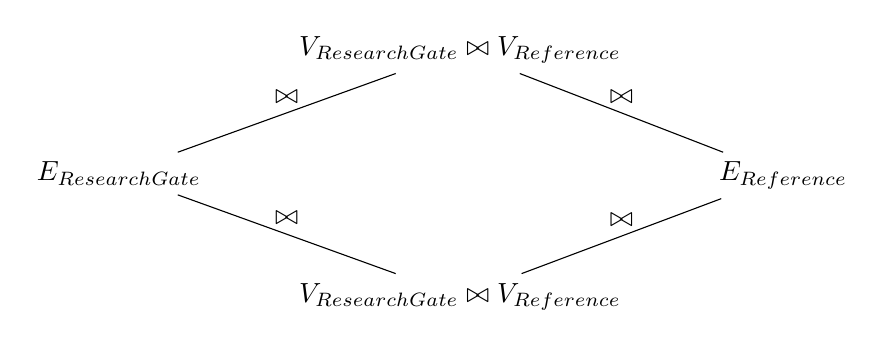
\begin{tikzpicture}[
    level/.style={sibling distance=2cm,
    level distance = 1cm}
]
    \tikzset{level 1/.style={sibling distance=4.5cm}}
    \node (a) {$V_{ResearchGate}\bowtie V_{Reference}$};
    \node[below left=of a] (l) {$E_{ResearchGate}$};
    \node[below right=of a] (r) {$E_{Reference}$};
    \node[below right=of l] (b) {$V_{ResearchGate}\bowtie V_{Reference}$};
    \path (a) edge node [midway,above] {$\bowtie$} (l);
    \path (a) edge node [midway,above] {$\bowtie$} (r);
    \path (b) edge node [midway,above] {$\bowtie$} (l);
    \path (b) edge node [midway,above] {$\bowtie$} (r);
\end{tikzpicture}
\end{document}